\documentclass[a4paper,12pt]{article} 

%Гралусы
\usepackage{gensymb}

%Система единиц СИ
\usepackage{siunitx}

%Добавляет возможность искать и копировать текст
\usepackage{cmap}

%Убирает пробел между названием таблицы/рисунка и самой таблицей/рисунком
\usepackage{caption}
\captionsetup[table]{skip= -0 cm}
\captionsetup[figure]{skip= -0 cm}

%Выравнивание названия таблиц по левому краю
%\usepackage[nooneline]{caption} 
%Размеры отступов 
\usepackage[left=20mm, top=20mm, right=20mm, bottom=20mm, footskip=10mm]{geometry}

%Рисунки
\usepackage{graphicx}
\usepackage{wrapfig} %обтекание элементов
\graphicspath{{graphs}{figures}}  % папки с картинками

%Русский язык в формулах
%\usepackage{mathtext}

%  Русский язык
\usepackage[T2A]{fontenc}			
\usepackage[utf8]{inputenc}			
\usepackage[english,russian]{babel}	

%Готические буквы
\usepackage{amssymb}

%Русский язык в формулах
\usepackage{mathtext}

% Математика
\usepackage{amsmath,amsfonts,amssymb,amsthm,mathtools} 
\usepackage{wasysym}

%Цветные подписи в таблице
\usepackage[table,xcdraw]{xcolor}

\usepackage{fancyhdr} % Колонтитулы
 	\pagestyle{fancy}
 	\renewcommand{\headrulewidth}{0.3mm}  % Толщина линейки, отчеркивающей верхний колонтитул
 	%\lfoot{Нижний левый}
 	%\rfoot{Нижний правый}
 	\rhead{Кафедра квантовой электроники}
 	%\chead{Верхний в центре}
 	\lhead{Белостоцкий А.И}
 	% \cfoot{Нижний в центре} % По умолчанию здесь номер страницы
 	
\begin{document} 

%Титульник 
\begin{titlepage}
	\begin{center}
		\large 	МИНИСТЕРСТВО ОБРАЗОВАНИЯ И НАУКИ РОССИЙСКОЙ ФЕДЕРАЦИИ\\
				МОСКОВСКИЙ ФИЗИКО-ТЕХНИЧЕСКИЙ ИНСТИТУТ \\
				(НАЦИОНАЛЬНЫЙ ИССЛЕДОВАТЕЛЬСКИЙ УНИВЕРСИТЕТ)\\ 
				ФИЗТЕХ-ШКОЛА ЭЛЕКТРОНИКИ, ФОТОНИКИ \\
				И МОЛЕКУЛЯРНОЙ ФИЗИКИ \\
		
		
		\vspace{4.0 cm}
		\LARGE{Отчет по лабораторной работе} \\ 
		\LARGE \textbf{Пространственные характеристики излучения полупроводникового инжекционного лазера} \\
	\end{center}
	\vspace{3 cm} \large

	%Надо подумать как это нормально написать	
	\begin{flushleft}
		Работу выполнил \hspace{5.5cm}  \underline{\hspace{3cm}} А.И.Белостоцкий \\	
		\vspace{2cm}
		Работу принял, оценка \hspace{4.3cm} \underline{\hspace{3cm}}
	\end{flushleft}
	
	
	\vfill

	\begin{center}
	Долгопрудный, 2023 г.
	\end{center}
\end{titlepage}           

\tableofcontents

\newpage

\section{Аннотация}

В данной работе будут исследованы диаграммы направленности излучения двух полупроводниковых инжекционных лазеров (ПИЛ). По полученным данным будет оценена толщина активного слоя каждого из образцов

\section{Экспериментальная установка} 

\begin{figure}[h!]
	\centering
	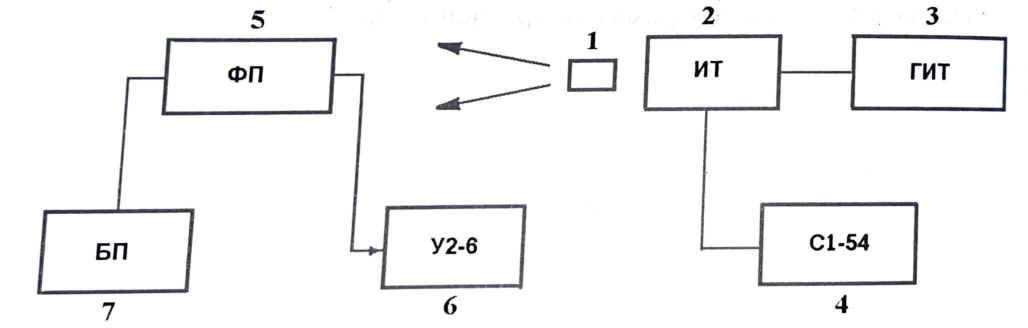
\includegraphics[width=\linewidth]{setup}
	\caption{Схема экспериментальной установки. (1) -- образец, (2) -- импульсный трансформатор, (3) -- генератор импульсов, (4) -- осциллограф, (5) -- фотоприемник, (6) -- микровольтметр, (7) -- блок питания.}
\end{figure}

\section{Теоретические сведения}

Рассмотрим диаграмму направленности ПИЛ

Если толщина активного слоя $d \gg \frac{\lambda}{2n_2}$ много больше длины волны излучения в активном слое, то можно считать, что коэффициент отражения выходного зеркала близок к френелевскому, а распределение поля на зеркальной грани резонатора такое же, как и внутри волновода. Распределение интенсивности излучения на зеркальной грани принято называть картиной ближней зоны

Распределение интенсивности по углам, т.е. диаграмма направленности, определяет картину дальней зоны. Это предполагает, что имеет место дифракция в параллельных лучах -- дифракция Фраунгофера. Отсюда следует, что расстояние $R$ до точки наблюдения должно выбираться из условия: размер тела свечения $D$ существенно меньше, чем первая зона Френеля. Нетрудно показать, что это требование приводит к соотношению $R \gg \frac{D^2}{\lambda}$

Для случая, когда поле внутри активного слоя диэлектрического волновода близко к полю внутри металлического волновода. Тогда выражение для амплитуды волны:

\begin{align*}
	S(\varphi) \sim \frac{\cos \left( \frac{\pi d}{\lambda} \sin \varphi \right) }{\left( \frac{\lambda(m+1)}{2d}\right)^2 - \sin^2 \varphi} \text{-- четные моды} \\
	S(\varphi) \sim \frac{\sin \left( \frac{\pi d}{\lambda} \sin \varphi \right) }{\left( \frac{\lambda(m+1)}{2d}\right)^2 - \sin^2 \varphi} \text{-- нечетные моды}
\end{align*}

\newpage

При $m=0$ диаграмма направленности имеет один главный максимум. Нетрудно показать, что:

\begin{equation} \label{eq:1}
	d = \frac{\lambda}{2 \sin \varphi_{0.6}},
\end{equation}

где $\varphi_{0.6}$ -- угол, такой что $I(\varphi_{0.6}) = 0,6 I(0)$

\section{Ход работы}

В эксперименте мы измеряем показания фотоприёмника -- $U$ -- причем $U \sim I$, следовательно угол $\varphi_{0.6}$ удовлетворяет соотношению $U(\varphi_{0.6}) = 0,6 U(0) = 0.6 U_{max}$ 

Перваый образец может быть помещен в установку 2 способами -- когда плоскость p-n--перехода параллельна щели (далее -- "Горизонтальная ориентация") и когда плоскость p-n--перехода перпендикулярна щели (далее -- "Вертикальная ориентация")
 
Вставим в установку первый образец горизонтально и снимем зависимость показаний фотоприемника от угла поворота образца -- результаты занесем в Таблицу 1.

\begin{table}[h!]
\centering
\caption{Зависимость сигнала фотоприемника от угла поворота первого образца в горизонтальной плоскости}
\begin{tabular}{|c|c|c|c|c|c|c|c|c|c|c|c|c|c|c|c|c|c|c|c|c|}
\hline
U, мВ & 510 & 600 & 640 & 660 & 690 & 700 & 720 & 720 & 720 & 750 \\ \hline
$\varphi, \degree$    & 9   & 8   & 7   & 6   & 5   & 4   & 3   & 2   & 1   & 0    \\ \hline
U, мВ & 745 & 740 & 720 & 720 & 700 & 690 & 680 & 660 & 640 & 320 \\ \hline
$\varphi, \degree$    & -1  & -2  & -3  & -4  & -5  & -6  & -7  & -8  & -9  & -10 \\ \hline
\end{tabular}
\end{table}

По полученным данным построим график зависимости $U = f(\varphi)$

\begin{figure}[h!]
	\centering
	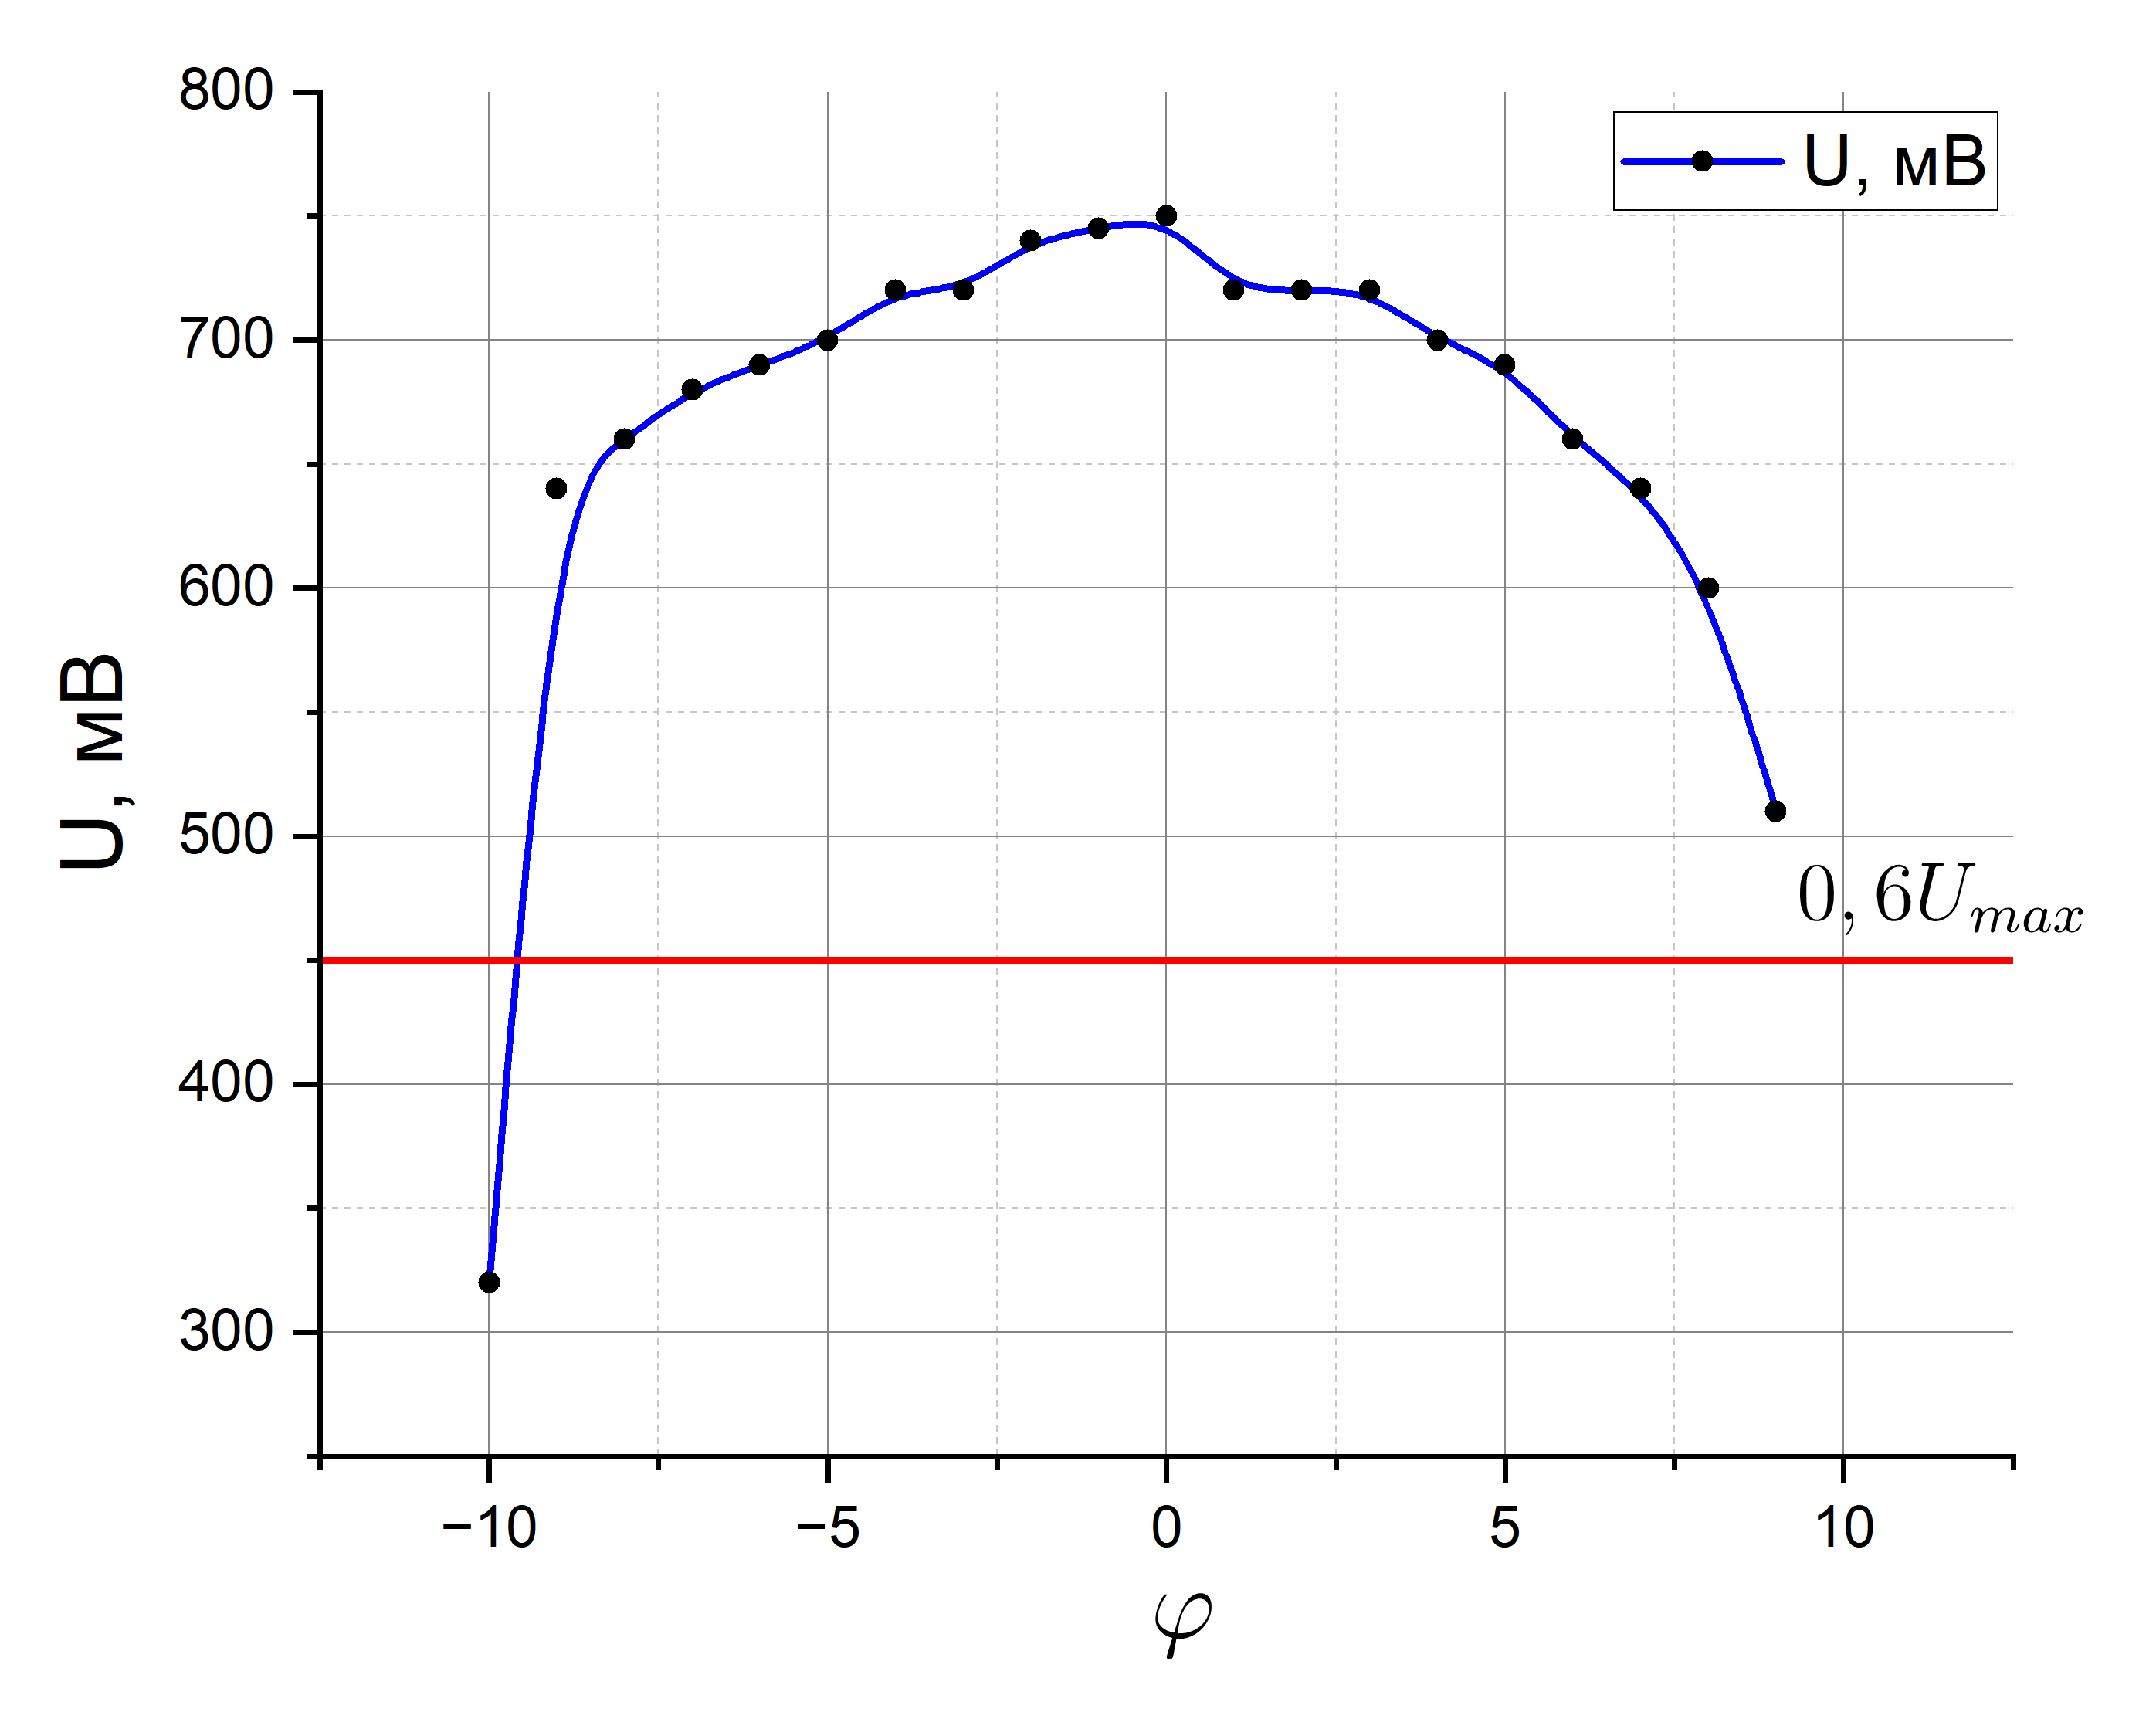
\includegraphics[width=0.8\linewidth]{Horizontal}
	\caption{Зависимость показаний фотоприемника от угла поворота (в градусах) первого образца для горизонтальной ориентации. Красным отмечена величина напряжения $0.6 U_{max}$}
\end{figure}

\newpage

Из резкого падения интенсивности -- можно сделать вывод, что значению сигнала фотоприемника при $\varphi = 10 \degree$ соответствует фоновая засветка. Учитывая это перестроим график:

\begin{figure}[h!]
	\centering
	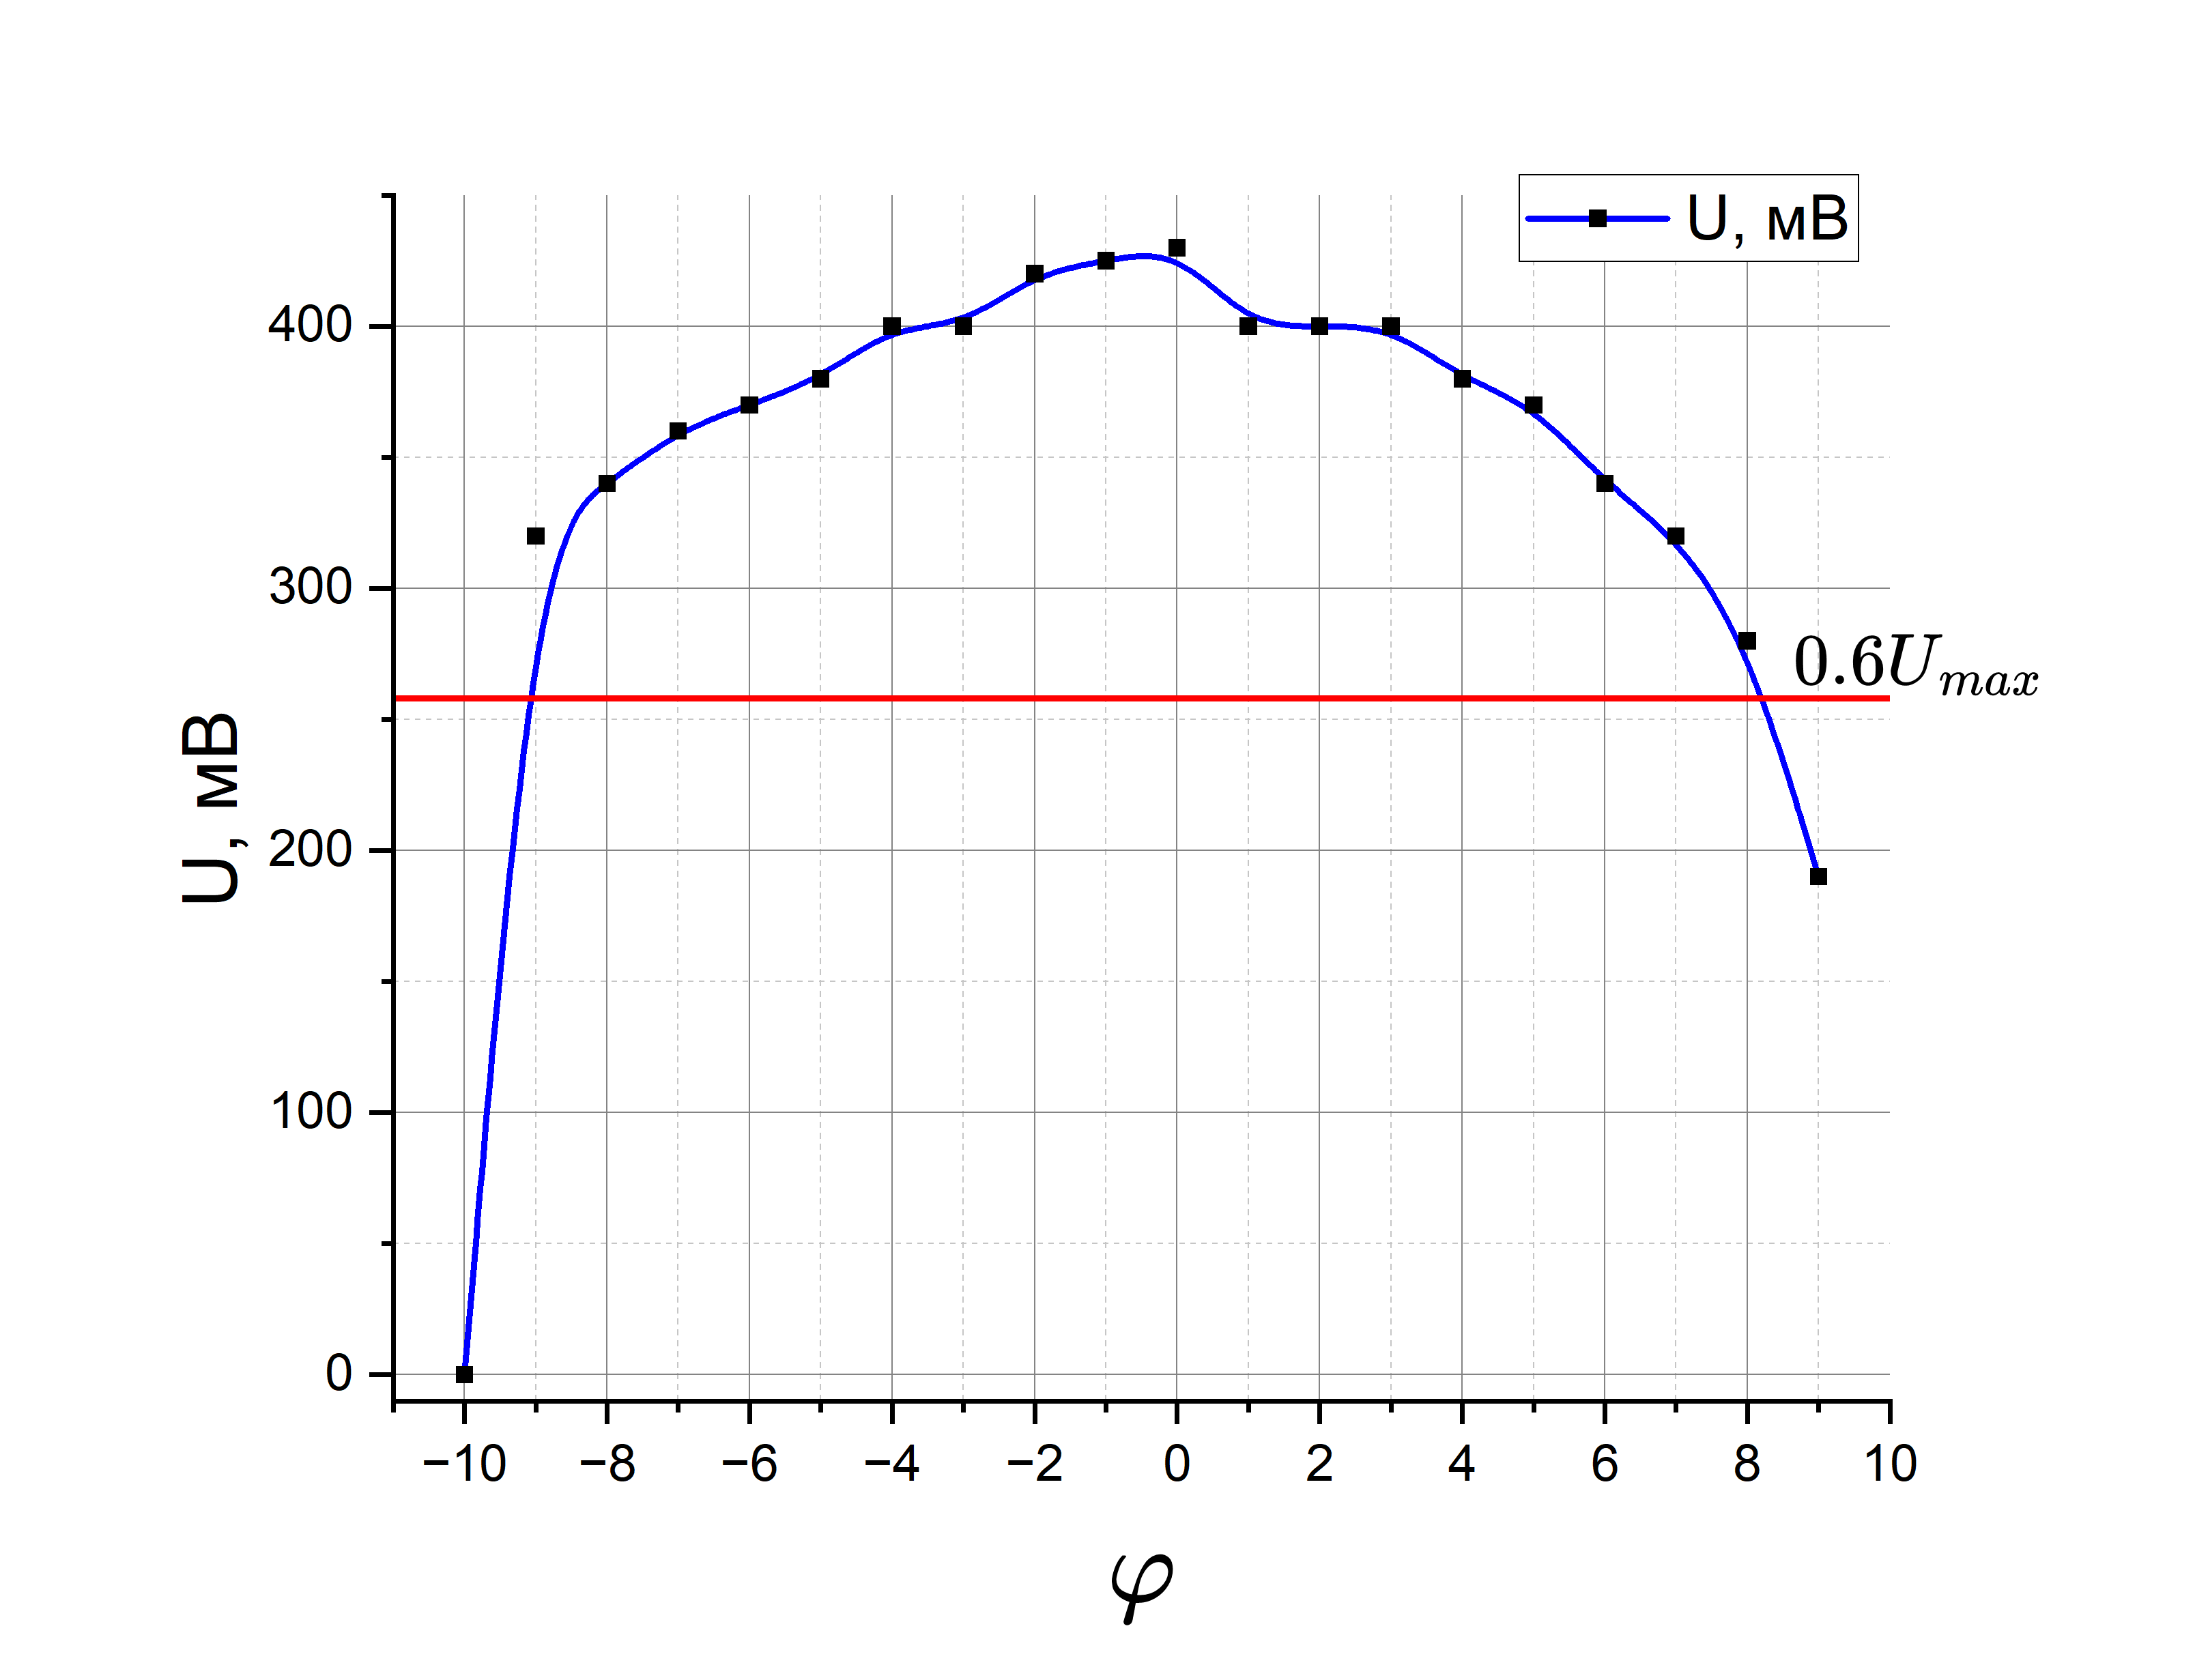
\includegraphics[width=0.95\linewidth]{Horizontal_2}
	\caption{Зависимость показаний фотоприемника от угла поворота (в градусах) первого образца для горизонтальной ориентации. Красным отмечена величина напряжения $0.6 U_{max}$}
\end{figure}

Оценим толщину активного слоя. Угол, отвечающий $0.6U{max}$ будем считать $\varphi \sim 10 \degree$. Тогда

$$
	d_{h} = \frac{\lambda}{2 \sin \varphi} \sim \frac{650}{2 \cdot 0,17 } \approx 1,9 \text{мкм}
$$

\newpage

Вставим в установку первый образец вертикально и снимем зависимость показаний фотоприемника от угла поворота образца -- результаты занесем в Таблицу 2.

\begin{table}[h!]
\centering
\caption{Зависимость сигнала фотоприемника от угла поворота первого образца в вертикальной плоскости.}
\begin{tabular}{|c|c|c|c|c|c|c|c|c|c|c|c|c|c|c|c|c|c|c|c|c|}
\hline
U, мВ & 140 & 230 & 460 & 520 & 690 & 790 & 780 & 680 & 590 & 400 & 200 & 130 \\ \hline
$\varphi, \degree$    & 5   & 4   & 3   & 2   & 1   & 0   & -1  & -2  & -3  & -4  & -5  & -6  \\ \hline
\end{tabular}
\end{table}

По полученным данным построим график зависимости $U = f(\varphi)$

\begin{figure}[h!]
	\centering
	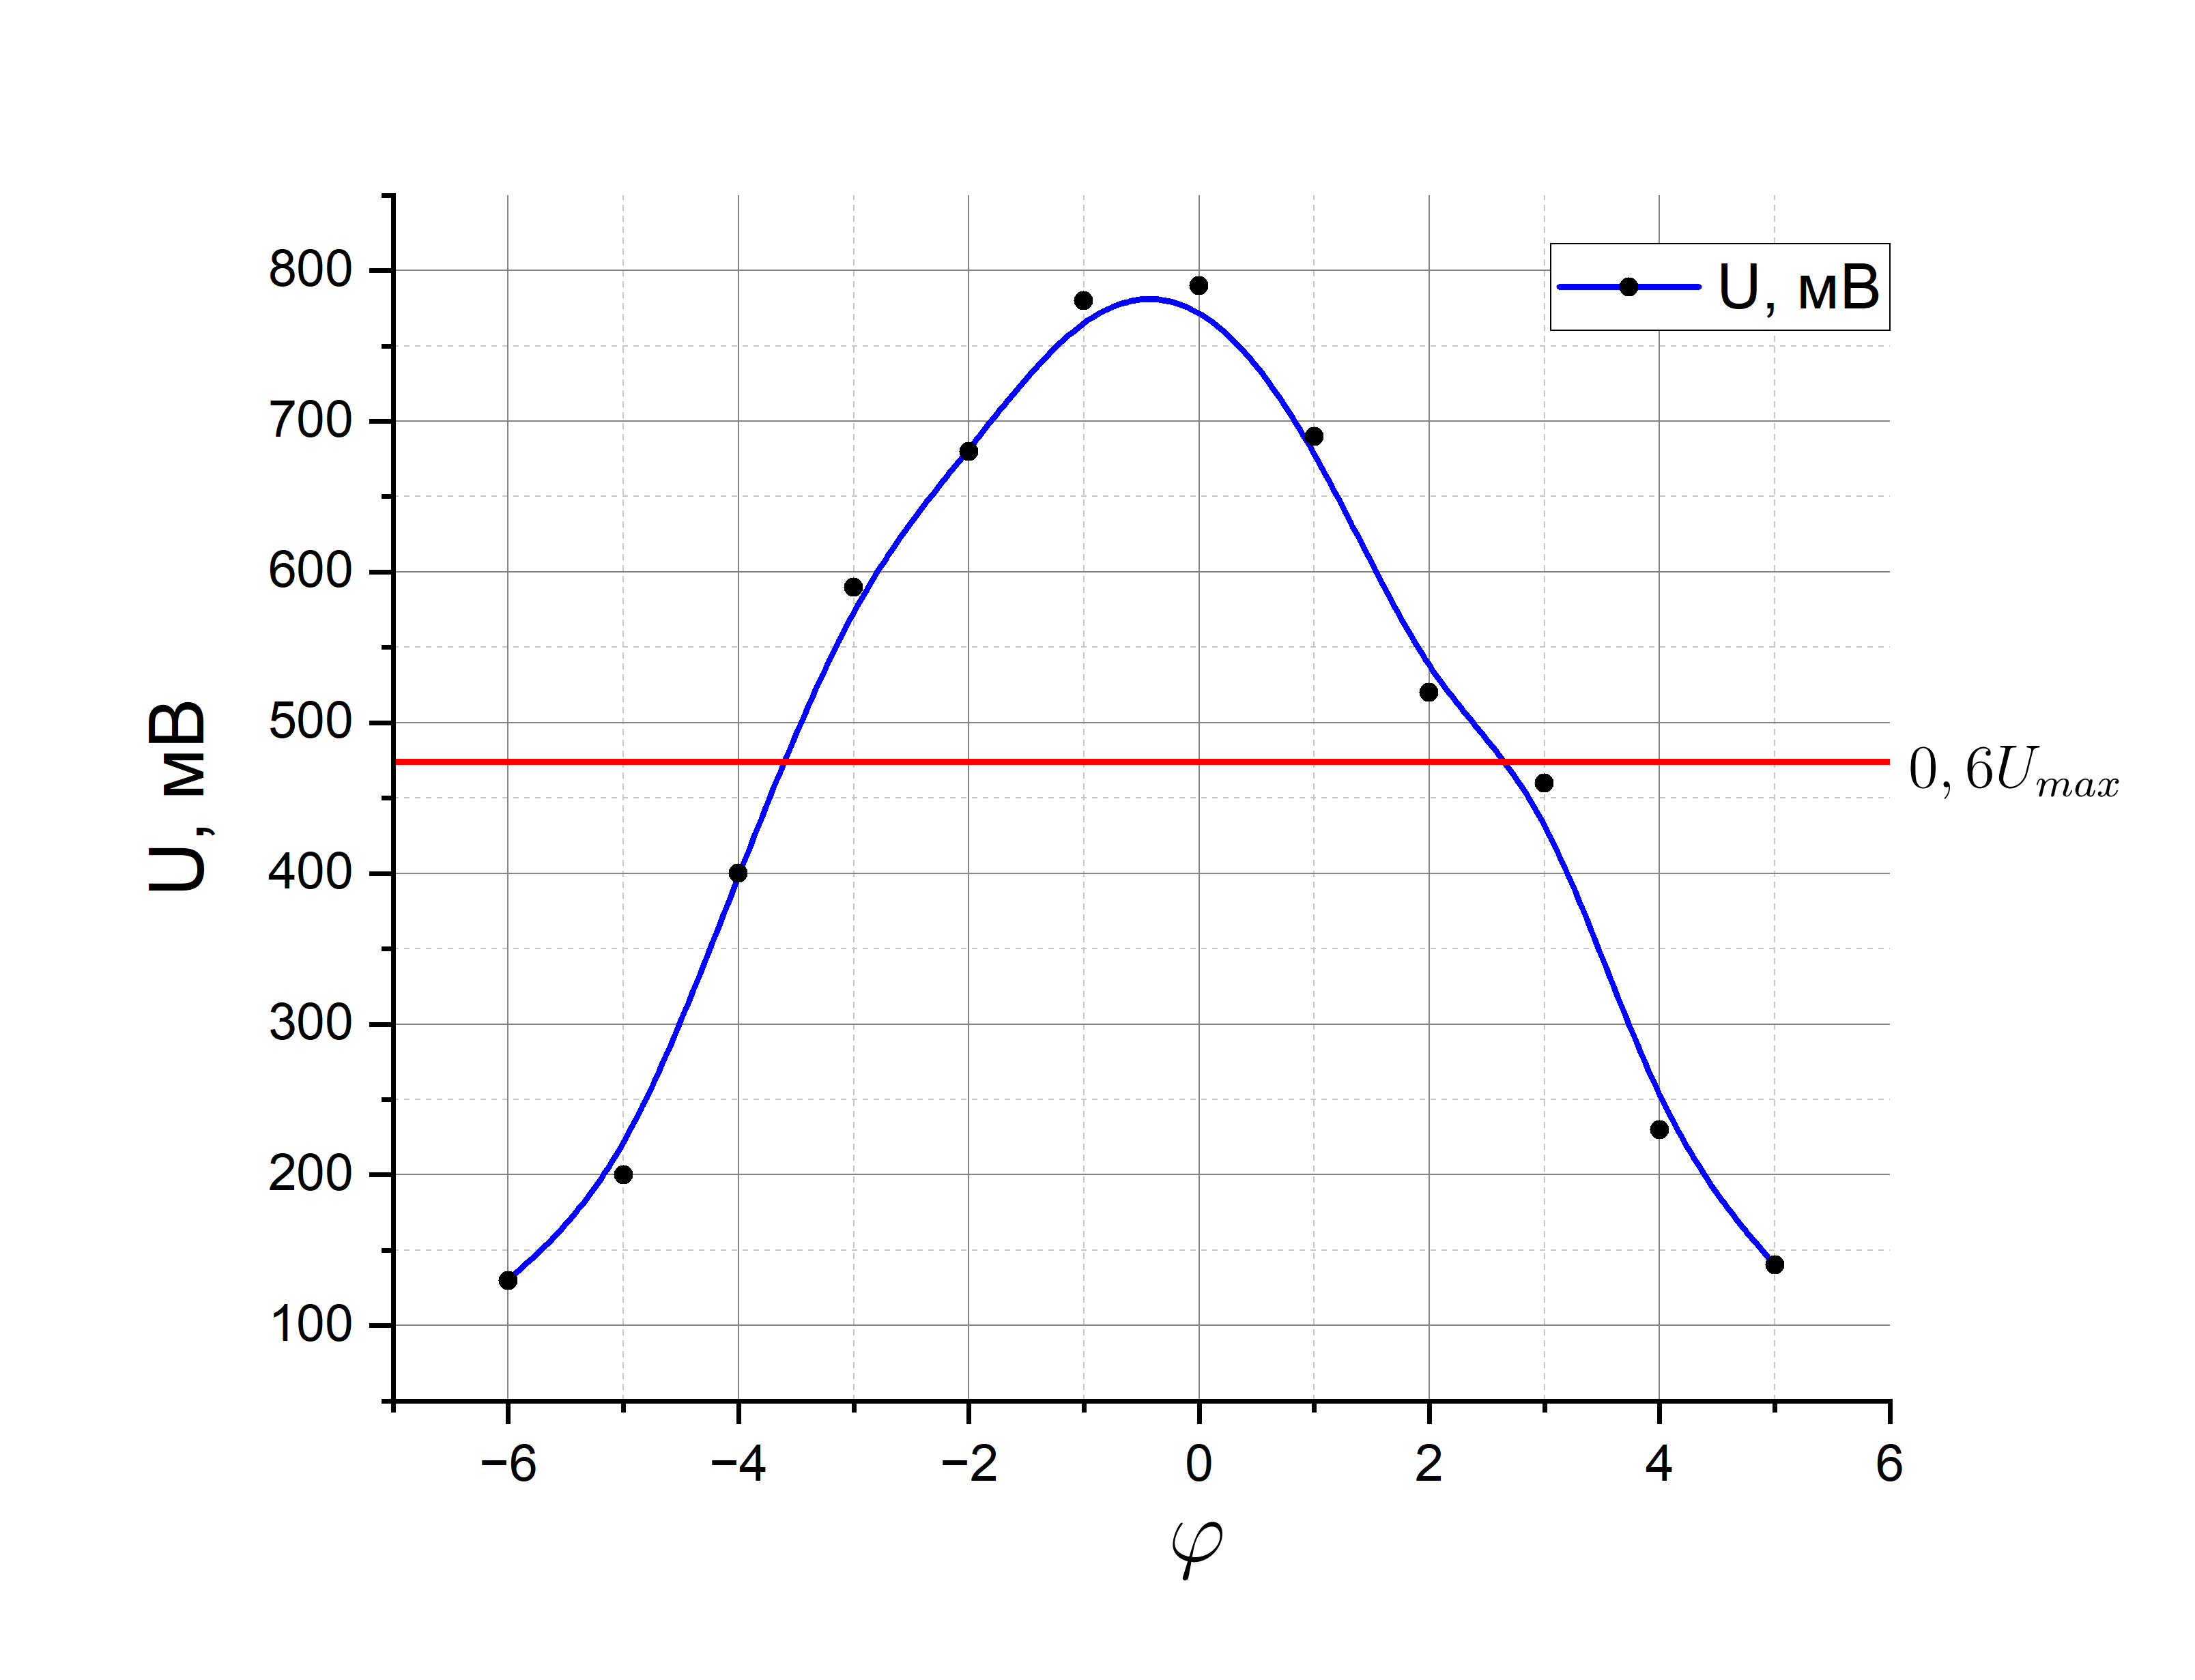
\includegraphics[width=0.95\linewidth]{Vertical}
	\caption{Зависимость показаний фотоприемника от угла поворота (в градусах) первого образца для вертикальной ориентации.Красным отмечена величина напряжения $0.6 U_{max}$}
\end{figure}


Оценим толщину активного слоя. Угол, отвечающий $0.6U{max}$ будем считать $\varphi \sim 3 \degree$. Тогда

$$
	d_{v} = \frac{\lambda}{2 \sin \varphi} \sim \frac{650}{2 \cdot 0,05 } \approx 6,5 \text{мкм}
$$

\newpage

Вставим в установку второй образец (пятно симметричное, поэтому не важно как мы его вставим) и снимем зависимость показаний фотоприемника от угла поворота образца -- результаты занесем в Таблицу 3.

\begin{table}[h!]
\centering
\caption{Зависимость сигнала фотоприемника от угла поворота второго образца}
\begin{tabular}{|c|c|c|c|c|c|c|c|c|c|c|c|c|c|c|c|c|c|c|c|c|}
\hline
U, мВ & 12 & 12 & 20 & 33 & 56 & 72 & 93 & 100 & 100 & 96 & 80 & 60 & 40 & 19 & 14 & 12 & 10 & 7   \\ \hline
$\varphi, \degree$    & 7  & 6  & 5  & 4  & 3  & 2  & 1  & 0   & -1  & -2 & -3 & -4 & -5 & -6 & -7 & -8 & -9 & -10 \\ \hline
\end{tabular}
\end{table}

По полученным данным построим график зависимости $U = f(\varphi)$

\begin{figure}[h!]
	\centering
	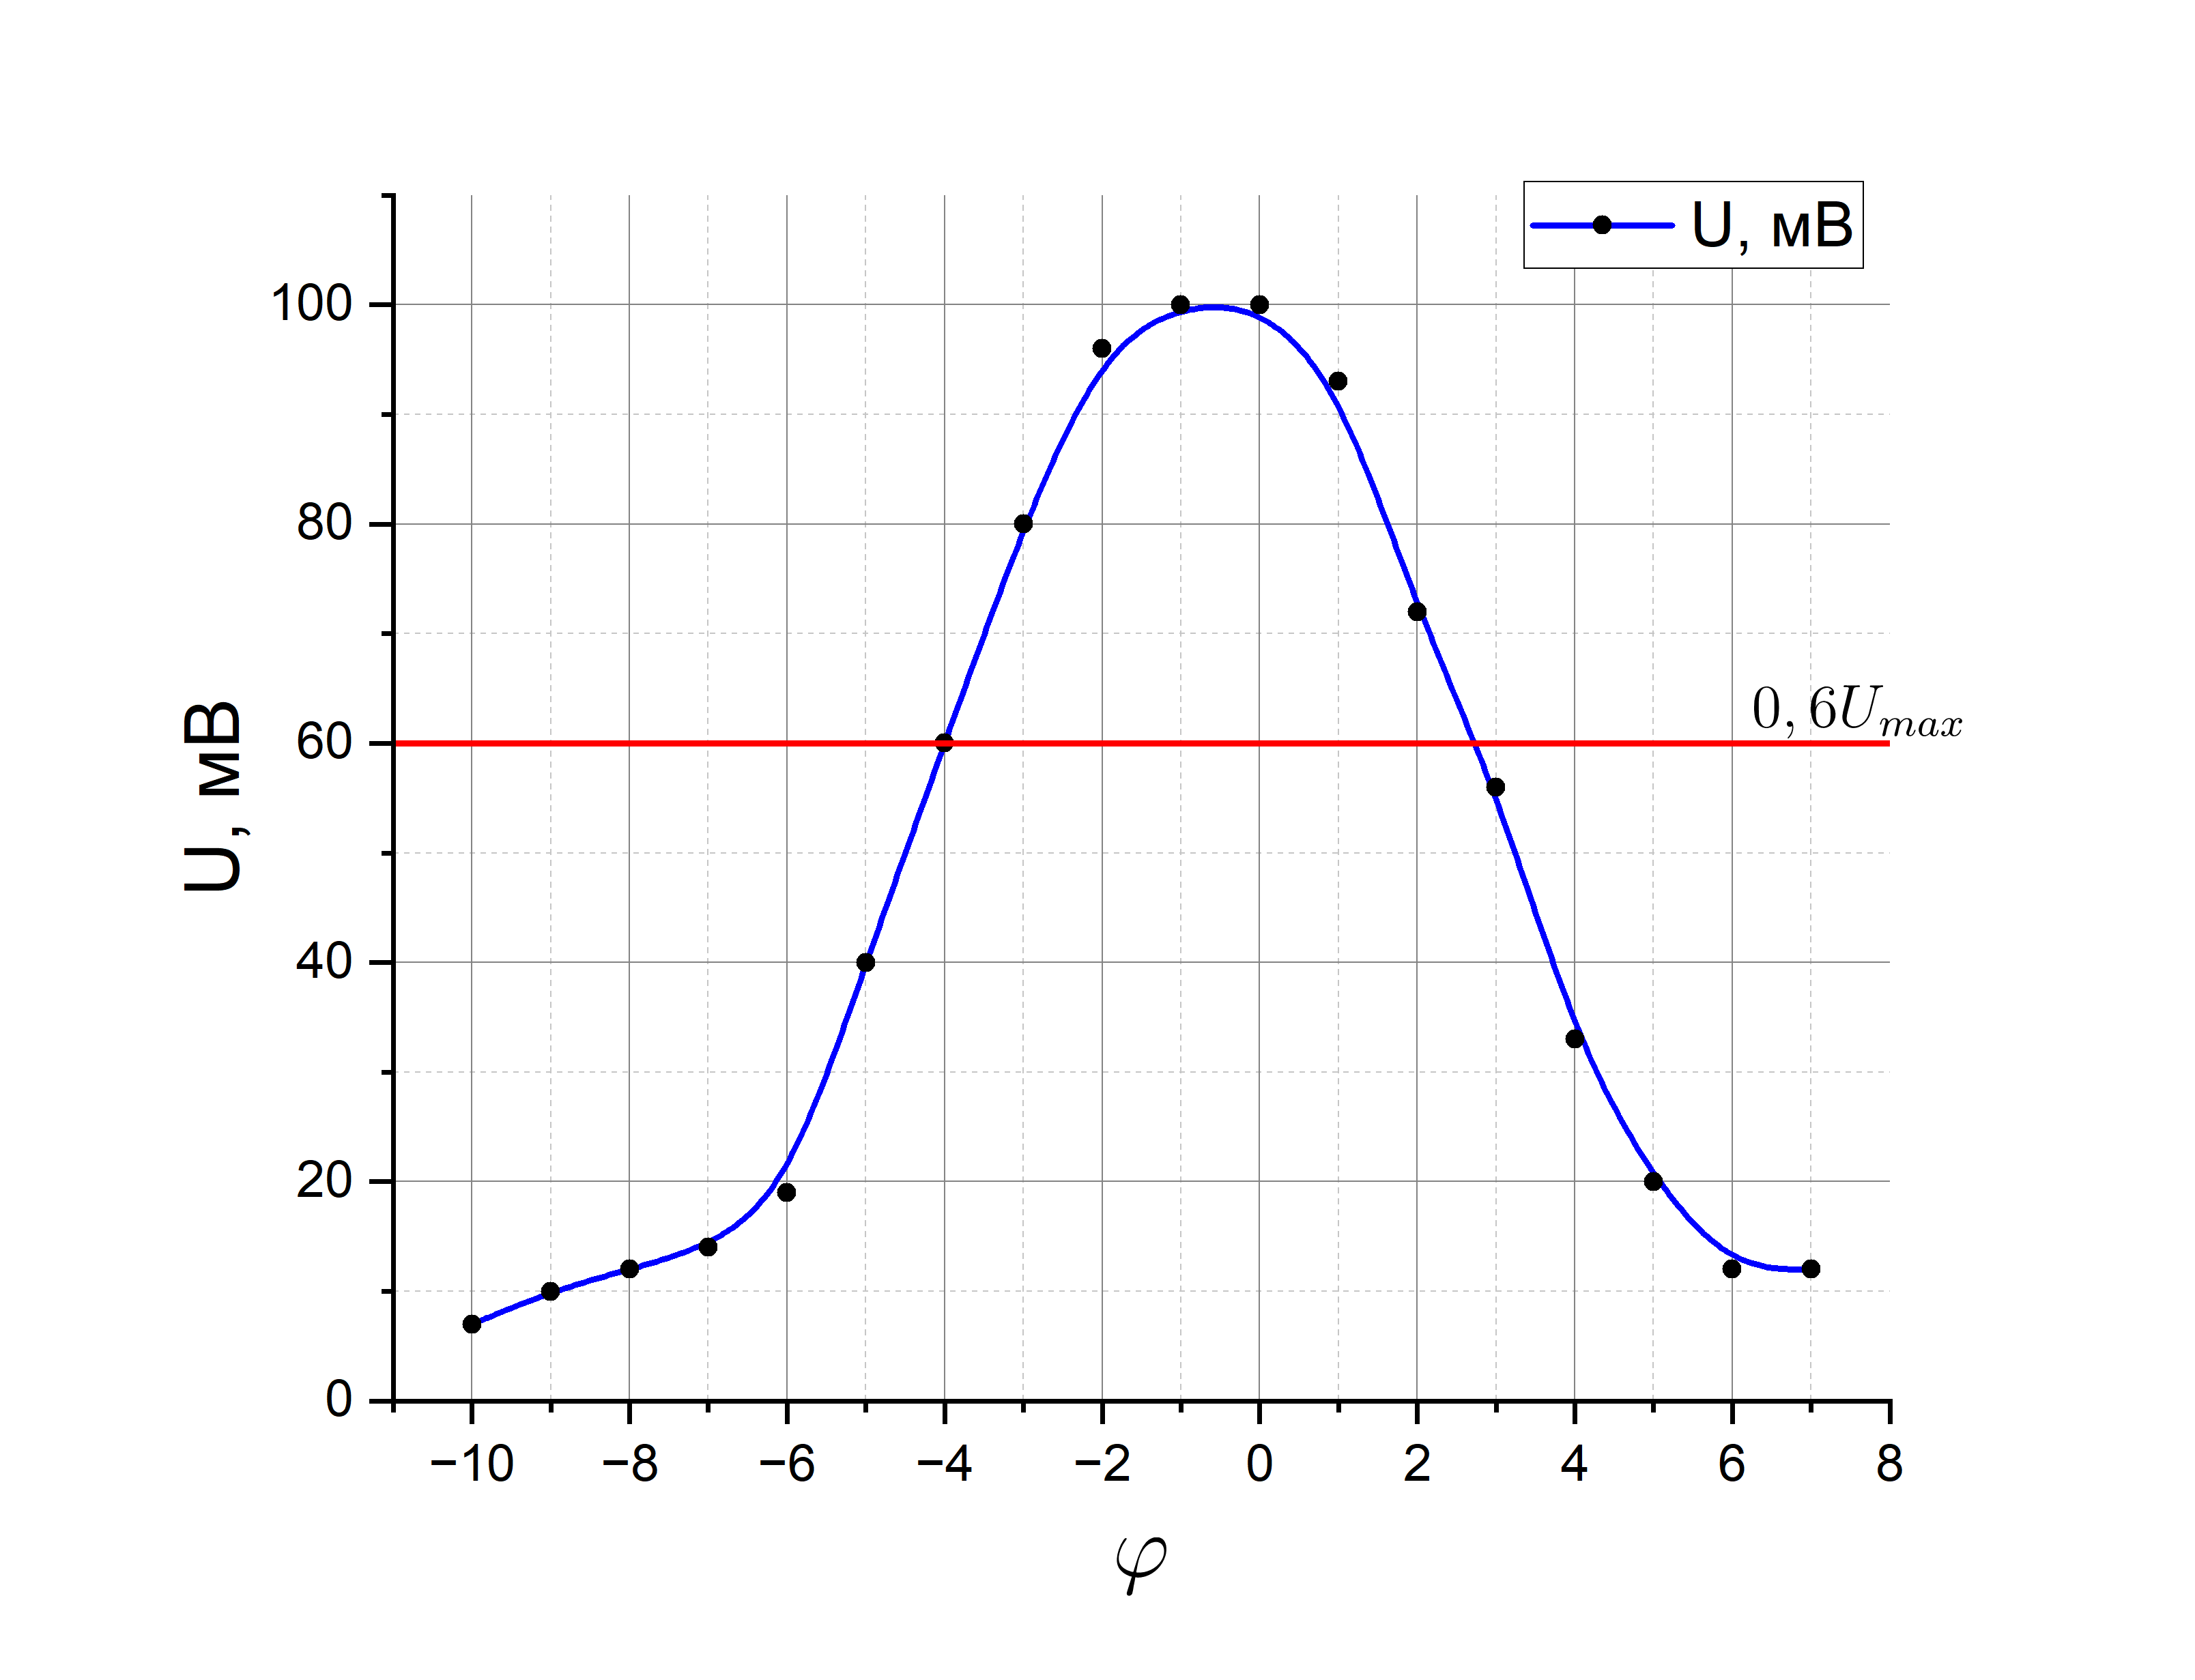
\includegraphics[width=0.95\linewidth]{Diod}
	\caption{Зависимость показаний фотоприемника от угла поворота (в градусах) второго образца.}
\end{figure}

Применяя теорию волноводов и излучения ПИЛ может быть рассчитана толщина активного слоя ПИЛ с данной диаграммой направленности.

$$
	d_{diod} = \frac{\lambda}{2 \sin \varphi} \sim \frac{650}{2 \cdot 0,17 } \approx 4,7 \text{мкм}
$$

\newpage

\section{Обсуждение результатов}

В результате данной работы были измерены диаграммы направленности для двух образцов, была оценена толщина активного слоя для первого образца. Также, по диаграмме направленности второго образца была оценена ширина активного слоя для ПИЛ, имеющего приведенную диаграмму направленности

\begin{table}[h!]	
	\centering
	\begin{tabular}{|c|c|c|c|}
	\hline
	       & Горизонтальная ориентация & Вертикальная ориентация & <<Диод>>\\ \hline
	d, мкм & 1,9                       & 6,5                     &   4,7\\ \hline
	\end{tabular}
\end{table}                             


\end{document}